\documentclass{article}
\usepackage{amssymb}
\usepackage{pdfpages}
\usepackage{hyperref}
\usepackage{cleveref}
\usepackage{enumitem}
% set the margin of the document
\usepackage[a4paper, total={7in, 10in}]{geometry}

\hypersetup{
	colorlinks=true,
	allcolors=blue,
}

\renewcommand{\thesubsection}{\thesection.\Alph{subsection}}


\begin{document}
\begin{titlepage}
   \vspace*{270px}
  \begin{center}

    \Large\textbf{CS446 Deliverable 5 - Architecture and Design Document}

   \vspace{50px}

    \Large{Project Title: Pitch-Perfectly-Accurately Practice}

   \vspace{50px}

    \large{Irvine Yao (b6yao)\\Jialin Shan (j6shan)\\Alex Lai \ (x7lai)\\Johnny Gao (z53gao)}

  \end{center}
\end{titlepage}
  
% set global enumerate line space
\setlist[enumerate]{topsep=0pt,itemsep=-1ex,partopsep=1ex,parsep=1ex}.
% set global itemize line space
\setitemize{noitemsep,topsep=0pt,parsep=0pt,partopsep=0pt}


\section{Architecture}
\label{sec:architecture}
\qquad
In order to fulfill our app’s main functionality, the following general architecture logic of our application is the following. First, we display the questions according to the modes users are currently using. The user can further customize what questions that they want to have asked by using the filter page. Then user will try to sing the correct note that is asked of them. Our app will constantly listen to the user through listeners with the mic. Once we got the sound data we will send the data to our library to get the current frequency to check whether user is singing the correct note or not. During the sound detection, we will display a bouncing arrow, asking the user to sing higher or lower. Based on our how our algorithm processes the data sent back from the library, we will display the result accordingly and if the answer is correct, we will display the next question. Otherwise, user can switch mode freely between note practice, interval practice, and triad mode, and our question page will be updated and generate question accordingly. 

In order to handle the sound data transmission between users, the result checking algorithm, and the library for sound frequency, we implemented the Model View Controller architecture (figure) as our main backend structure.

In our MVC architecture framework, Controller is the component where most of the application’s algorithms and logic reside, and is able to manipulate model and update view. Model component have all the data and objects we need for the data transmission within the app. It is inert component where if no one calls it, it will not do anything, and provide data to controller.  View is a component that can interact with user, having layouts, views for displaying information, Microphone for gathering sound data, and Noteplayer for playing sound to user. 

The reason we choose MVC architecture style for our app is because our app is highly interactive. So  in order for users to see real time respond right when the user produce voice, we need  model can help us store history of what user sings, and having the controller as the central processing unit enables it to modify model and update view in real time. Model-view-controller is the best choice.

Once our application has started, our Controller component will generate the question based on our default settings data from the Model component, then send them to the viewer component of our architecture. In our view component, we will set up layouts and text, and a runnable thread in our VoiceListener class by utilizing a method from the Tarsos library, the library we use to handle the sound signal data. The library creates a thread that will be used for constantly getting data from the microphone and generate the correct current frequency from the data. The user will see the question through the Viewer component and try to provide the answer to controller component, by singing to the microphone connecting to our view component. Once the view component get the sound data, it will generate the frequency of the current sound and send this data to the Controller component in real-time for frequency processes. In our Controller component, we have multiple internal logics and algorithms that will decide whether the current note our user is singing is too high, too low or is in the target frequency range, and will update the viewer component in real-time accordingly. Here are two possible scenarios:

Scenario 1:
A Microphone (view) is where user can input voice. Controller gets notified whenever current frequency stored in Microphone is changed. Controller then process the frequency and updates view the arrow suggestion (Note Practice Mode) or a real-time graph (Graph Mode). 

Scenario 2:
The user clicks on Mode button (e.g. Note Practice Mode) in navigation menu (view), the view notifies MainActivity (also controller). The MainActivity then change current Mode in Model. Since Controller (not MainActivity) subscribes to data changes in Model, Controller gets notified and then further interact with the Model. Finally, Controller updates view with texts from next Question.


In order to let the user to navigate between different modes, we created a left drawer containing 3 buttons corresponding to the modes in the viewer. Each mode will be represented as a Fragment in the Controller. Once the user wants to switch mode, they will interact with our user interface through their touch screen in the View. The view will then notify the Controller component which mode is requested, from which Controller then will update viewer correspondingly.

To implement filter page, we utilize pipe and filter (figure) as architecture style. At first, we have a bitmap with 88 “1”s, representing all 88 notes, which are all the musical notes available. Once user finishes selecting their preference on different spinner on the filter page, we pass our initial bitmap to a series of filters one by one to get the final result, like a pipe line. For example, if you are in note practice mode’s filter page, our backend will automatically have two filter, range and scale filter, ready. Then you will select the range of your preferred notes, scale and key signatures of the notes you want to practice. Every time you make a selection, the bitmap will go through those aforementioned filters to get the updated note pool, and display under the spinner. Finally, after user clicks the note that they don’t want to sing, we will have the result bitmap with all the note that has passed the filter, and waiting to be chosen as question.

For our question generation, we use inheritance class structure and polymorphism to manage our question classes. We first have an abstract question class containing all of the reusable methods and fields for every modes’ question. Then we implemented three question classes as the child class for each practice mode’s question. 
 
Our architecture design is also able to support most of the NFPs, such as scalability, maintainability and performance, aforementioned in the proposal documents. Thanks to the modularity of our overall architecture design, the scalability maintainability part of our NFP can be easily achieved. For example, If we would like to add more practice modes to our app later on, we could simply create corresponding fragments and their question class under their own higher abstract class, and that would be it. Also thanks to the advantage of MVC, we can maintain each component of MVC independently without disturbing the whole system. Last but not least, thanks to the clarity of our design and library utilize, our app is able to give real-time feedback while user singing without regard to your devices, achieving the performance and usability parts of NFP.


\section{Design}
\label{sec:Design}

\section{Visual explaination}
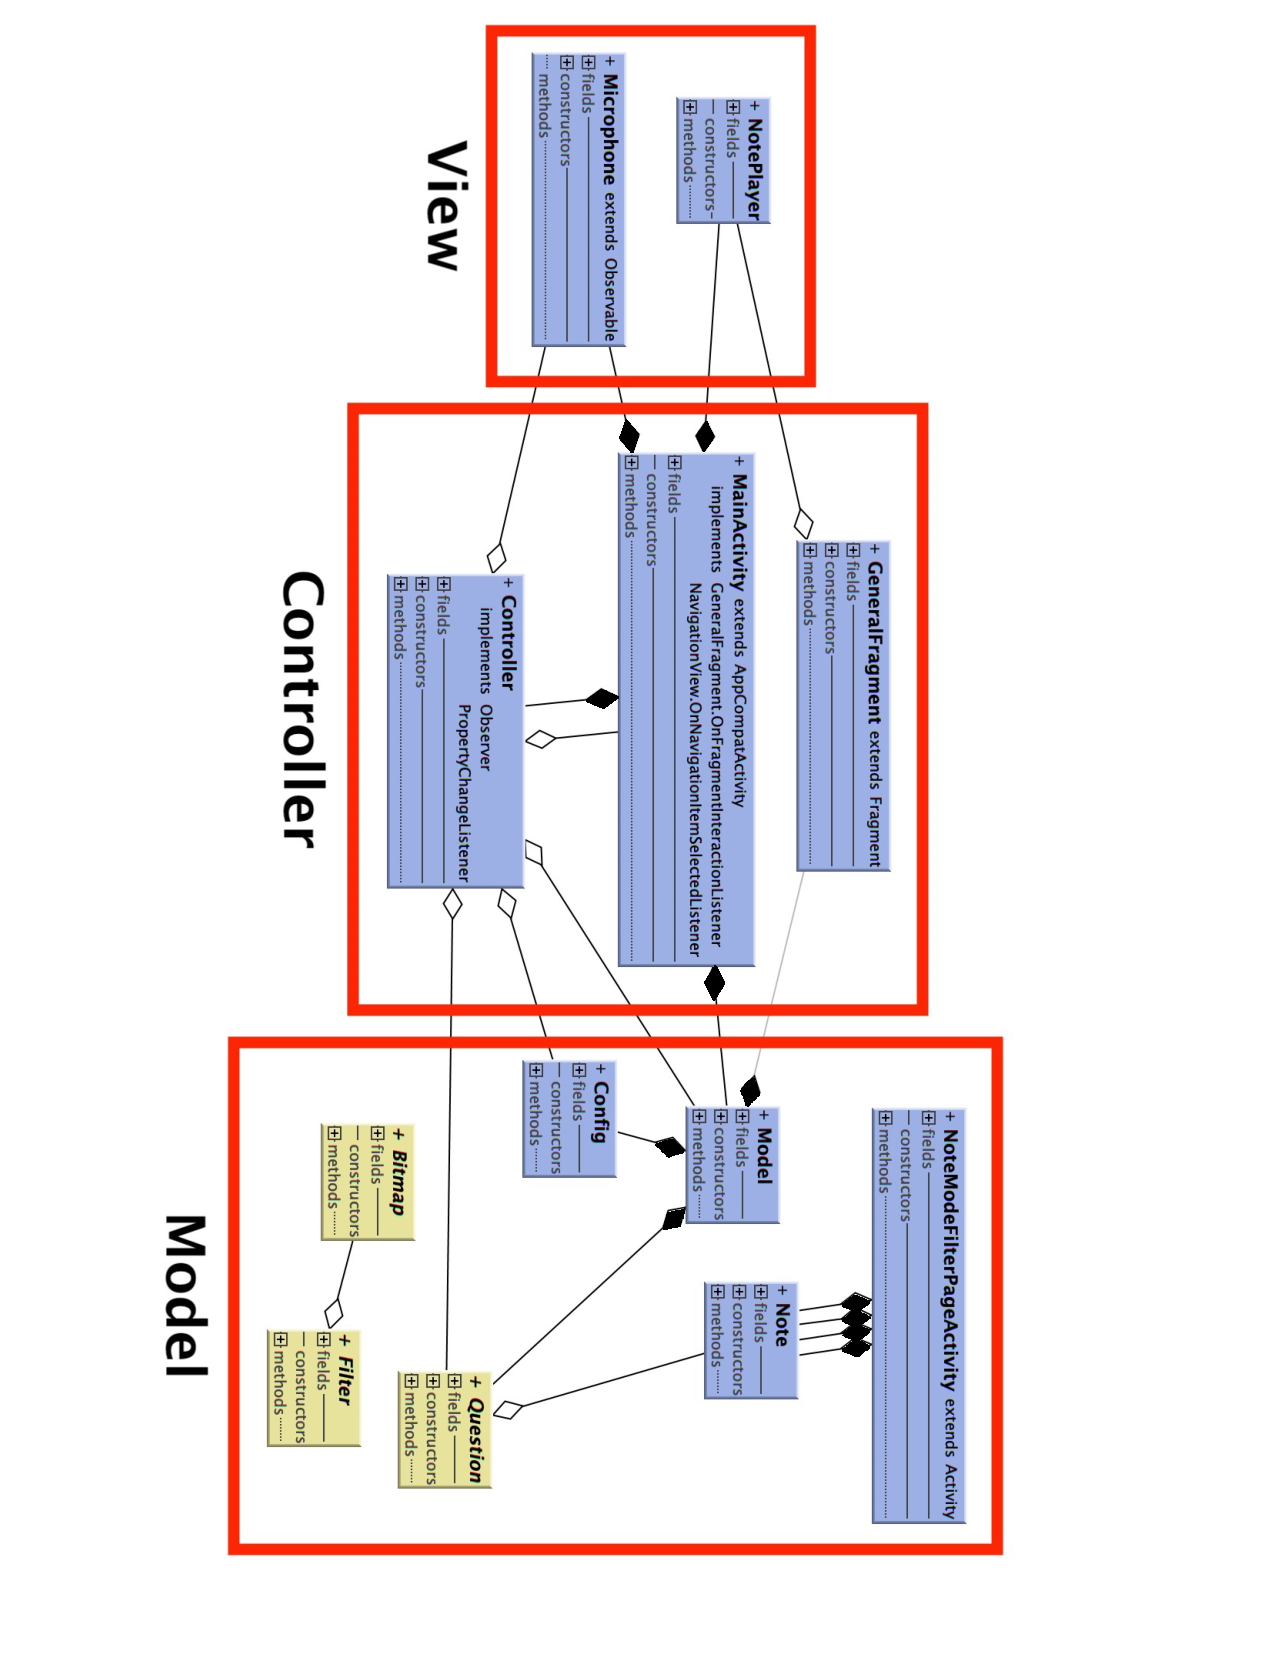
\includepdf[pages={1}]{./graph.pdf}
\includepdf[pages={2}]{./graph.pdf}

\end{document}
